\documentclass[a4paper,12pt]{article}
\usepackage{amsmath,amsfonts,amssymb,graphicx}
\usepackage[table,xcdraw]{xcolor}
\usepackage{array,geometry,longtable,booktabs,caption,authblk,orcidlink}
\usepackage{subcaption,pdflscape,tabularx,multirow,float,adjustbox,ragged2e}
\usepackage{hyperref}
\usepackage{tikz}
\usetikzlibrary{arrows.meta,positioning,shapes.geometric}
\geometry{a4paper,left=0.65in,right=0.65in,top=0.8in,bottom=0.8in}
\setlength{\parindent}{0pt}
\captionsetup[table]{skip=8pt}
\hypersetup{colorlinks=true,linkcolor=blue,citecolor=blue,urlcolor=blue}

\begin{document}

\title{Post-Myocardial-Infarction Survival Modelling from Echocardiographic Variables: Cox Regression, Fractional Polynomials, Random Survival Forests, and Synthetic-Data Augmentation}

\author[1]{Md Abu Sufian\orcidlink{0009-0007-3503-6942}}
\author[2]{Wahiba Hamzi}
\author[3]{Mai Ali\orcidlink{0000-0002-5907-6048}}
\author[4]{Amira Ali\orcidlink{0009-0000-3575-920X}}
\author[5,6,7]{Boumediene Hamzi\orcidlink{0000-0002-9446-2614}\thanks{Correspondence: b.hamzi@imperial.ac.uk}}

\affil[1]{University of East London, School of Architecture, Computing and Engineering, London, E16 2RD, UK, m.sufian@uel.ac.uk}
\affil[2]{Laboratoire de Biotechnologie Santé et Environnement, Department of Biology, University of Blida, Blida 09000, Algeria; hamzi.wahiba@univ-blida.dz}
\affil[3]{The Edward S. Rogers Department of Electrical and Computer Engineering, University of Toronto, Toronto, ON M5S 1A1, Canada, Maia.ali@mail.utoronto.ca}
\affil[4]{School of Medicine, Imperial College London, London SW7 2AZ, UK, amira.ali21@imperial.ac.uk}
\affil[5]{Department of Computing and Mathematical Sciences, California Institute of Technology, Caltech, CA 91125, USA}
\affil[6]{The Alan Turing Institute, London NW1 2DB, UK}
\affil[7]{Department of Mathematics, Imperial College London, London SW7 2AZ, UK}
\date{}
\maketitle

\begin{abstract}
\textbf{Background/Objectives:} The UCI Echocardiogram dataset is a small historical cohort describing survival after myocardial infarction (MI), rather than a heart-failure outcome. We re-evaluated post-MI survival using a reproducible analysis that separates the 132 original records from synthetic observations and directly compares conventional and machine-learning survival models.

\textbf{Methods:} The original 13-field UCI schema was reconstructed. Survival time was the number of months observed after MI; death was defined as the event and patients still alive at last observation were censored. Kaplan--Meier analysis used 130 records with valid survival/status data (88 deaths, 42 censored). Multivariable modelling used 107 complete cases (75 deaths) and six prespecified variables: age, pericardial effusion, fractional shortening, E-point septal separation (EPSS), left-ventricular end-diastolic dimension (LVDD), and wall-motion index (WMI). Cox proportional hazards (PH), nested fractional-polynomial Cox (FP-Cox), and Random Survival Forest (RSF) models were evaluated on identical repeated 5-fold cross-validation splits (5 repeats). Discrimination was quantified by the concordance index and prediction error by inverse-probability-of-censoring-weighted Brier scores at 12, 24, and 36 months and the integrated Brier score (IBS) over 6--36 months. A smoothed multivariate bootstrap was evaluated as an exploratory synthetic-data augmentation strategy, with generation confined to training folds and all utility assessed on held-out real observations.

\textbf{Results:} Kaplan--Meier survival was 91.7\% at 12 months, 70.1\% at 24 months, 26.6\% at 36 months, and 11.0\% at 48 months; median survival was 29 months. No covariate was statistically significant in the six-variable Cox model. The apparent Cox C-index was 0.532 and the bootstrap optimism-corrected value was 0.459. In repeated cross-validation, C-index/IBS were 0.443/0.170 for Cox, 0.432/0.171 for FP-Cox, and 0.446/0.167 for RSF. Fractional-polynomial transformations of age and WMI produced negligible improvement in full-sample AIC and unstable powers across folds. Synthetic augmentation preserved marginal and correlation structure but did not provide a robust performance benefit: real+1$\times$ synthetic Cox yielded C-index 0.457 but IBS 0.172.

\textbf{Conclusion:} In this small post-MI cohort, more flexible models did not materially outperform conventional Cox regression, and synthetic augmentation did not create additional clinical evidence. The revised analysis supports cautious methodological conclusions, emphasises transparent internal validation, and does not treat synthetic records as independent patients or external validation.

\textbf{Keywords:} myocardial infarction; survival analysis; echocardiography; Cox proportional hazards; random survival forest; fractional polynomials; synthetic data; internal validation.
\end{abstract}

\section{Introduction}
Cardiovascular disease remains a major cause of morbidity and mortality worldwide, and myocardial infarction can lead to acute and long-term complications through myocardial ischaemia, impaired ventricular function, arrhythmia, and haemodynamic instability \cite{ref1,ref3,ref4}. Survival analysis is therefore important when the clinical outcome is time from MI to death or censoring. The UCI Echocardiogram dataset was created for this purpose: it contains echocardiographic and clinical measurements obtained after MI together with observed survival time and vital status \cite{ref44}.

Cox proportional hazards regression remains a standard approach for time-to-event analysis because it provides interpretable hazard ratios without requiring a parametric baseline hazard \cite{ref30}. Its use nevertheless requires careful attention to proportional hazards and to the functional form of continuous predictors \cite{ref7,ref14}. Categorising continuous variables can discard information, whereas fractional polynomials provide a parsimonious way to assess departures from linearity \cite{ref10,ref36}. Random Survival Forests (RSF) offer a non-parametric alternative capable of modelling interactions and non-linear relationships without imposing proportional hazards \cite{ref38}.

The submitted version of this study combined the 132-record source cohort with a 100,000-record synthetic extension and consequently blurred the distinction between observed patients and generated observations. The present revision resolves that ambiguity. The real UCI cohort is the sole basis for clinical and statistical inference. Synthetic data are retained only as a methodological augmentation experiment, are explicitly labelled as artificial observations, and are never treated as additional patients or as external validation. This distinction is important because synthetic health data may be useful for augmentation or privacy-preserving development, but fidelity to source distributions does not increase the independent clinical information contained in the original cohort \cite{ref40,ref41}.

The objectives of the revised study were therefore to: (i) reconstruct the original UCI schema and define survival time, death events, and censoring unambiguously; (ii) estimate post-MI survival using Kaplan--Meier and multivariable Cox PH analysis; (iii) formally test nonlinear age and WMI relationships using fractional polynomials; (iv) compare Cox PH, FP-Cox, and RSF under identical repeated cross-validation with censoring-aware metrics; and (v) assess whether transparently generated synthetic observations improve predictive utility when evaluated exclusively on held-out real observations. We additionally report model instability and limitations rather than interpreting weak internal signals as established clinical effects.

\section{Methods}
\subsection{Data source, schema reconstruction, and outcome definition}
The analysis used the original UCI Echocardiogram dataset (132 records) \cite{ref44}. The raw file contains 13 fields in the following order: survival, still-alive, age at heart attack, pericardial effusion, fractional shortening, EPSS, LVDD, wall-motion score, wall-motion index, multiplicative factor, name, group, and alive-at-one-year. The revised parser retained this full schema and treated ``?'' as missing. The endpoint was post-MI survival: \texttt{survival} records months observed after MI, while \texttt{still\_alive}=0 denotes death and \texttt{still\_alive}=1 denotes a patient alive at the last recorded follow-up. The event indicator used by all survival models was therefore
\[
\text{event}=1-\texttt{still\_alive},
\]
so that event=1 indicates death and event=0 indicates right censoring.

The variable labelled PE in the original submission is correctly described here as \emph{pericardial effusion}, not pulmonary embolism. The primary predictor set comprised age, pericardial effusion, fractional shortening, EPSS, LVDD, and WMI. Wall-motion score was not entered simultaneously with WMI because WMI is a normalized wall-motion measure and inclusion of both would add redundancy. The UCI fields \texttt{mult}, \texttt{name}, and \texttt{group} were not used as predictors. The derived \texttt{alive\_at\_one} variable was not used as the continuous-time event indicator and had substantial missingness.

\subsection{Missing data and analysis populations}
Kaplan--Meier analysis used all records with valid survival time and vital status. Multivariable models used complete cases for survival, event status, and the six prespecified predictors; no imputation was performed for the primary analysis. This resulted in two analysis populations: 130 records for Kaplan--Meier estimation and 107 complete cases for multivariable modelling.

\begin{table}[H]
\centering
\caption{Observed data availability in the reconstructed UCI Echocardiogram dataset.}
\label{tab:missingness}
\begin{tabular}{lrr}
\toprule
Variable & Observed, n & Missing, n \\
\midrule
Survival time & 130 & 2 \\
Still alive / vital status & 131 & 1 \\
Age & 127 & 5 \\
Pericardial effusion & 131 & 1 \\
Fractional shortening & 124 & 8 \\
EPSS & 117 & 15 \\
LVDD & 121 & 11 \\
Wall-motion score & 128 & 4 \\
Wall-motion index & 131 & 1 \\
Multiplicative factor & 128 & 4 \\
Alive at one year & 74 & 58 \\
\bottomrule
\end{tabular}
\end{table}

\begin{table}[H]
\centering
\caption{Descriptive statistics from the reconstructed original cohort.}
\label{tab:descriptive}
\begin{adjustbox}{max width=\linewidth}
\begin{tabular}{lrrrrrr}
\toprule
Variable & n & Mean & SD & Median & Min & Max \\
\midrule
Survival (months) & 130 & 22.183 & 15.858 & 23.500 & 0.03 & 57.00 \\
Age (years) & 127 & 62.925 & 8.404 & 62.000 & 35.00 & 86.00 \\
Pericardial effusion & 131 & 0.183 & 0.388 & 0 & 0 & 1 \\
Fractional shortening & 124 & 0.217 & 0.108 & 0.205 & 0.01 & 0.61 \\
EPSS & 117 & 12.165 & 7.370 & 11.000 & 0.00 & 40.00 \\
LVDD & 121 & 4.763 & 0.810 & 4.650 & 2.32 & 6.78 \\
Wall-motion score & 128 & 14.438 & 5.019 & 14.000 & 2.00 & 39.00 \\
Wall-motion index & 131 & 1.383 & 0.453 & 1.222 & 1.00 & 3.00 \\
\bottomrule
\end{tabular}
\end{adjustbox}
\end{table}

\subsection{Analysis workflow}
Figure~\ref{fig:studyflow} summarises the revised analysis. Synthetic data were generated only after real-data preprocessing and only within model-training folds for predictive utility experiments.

\begin{figure}[H]
\centering
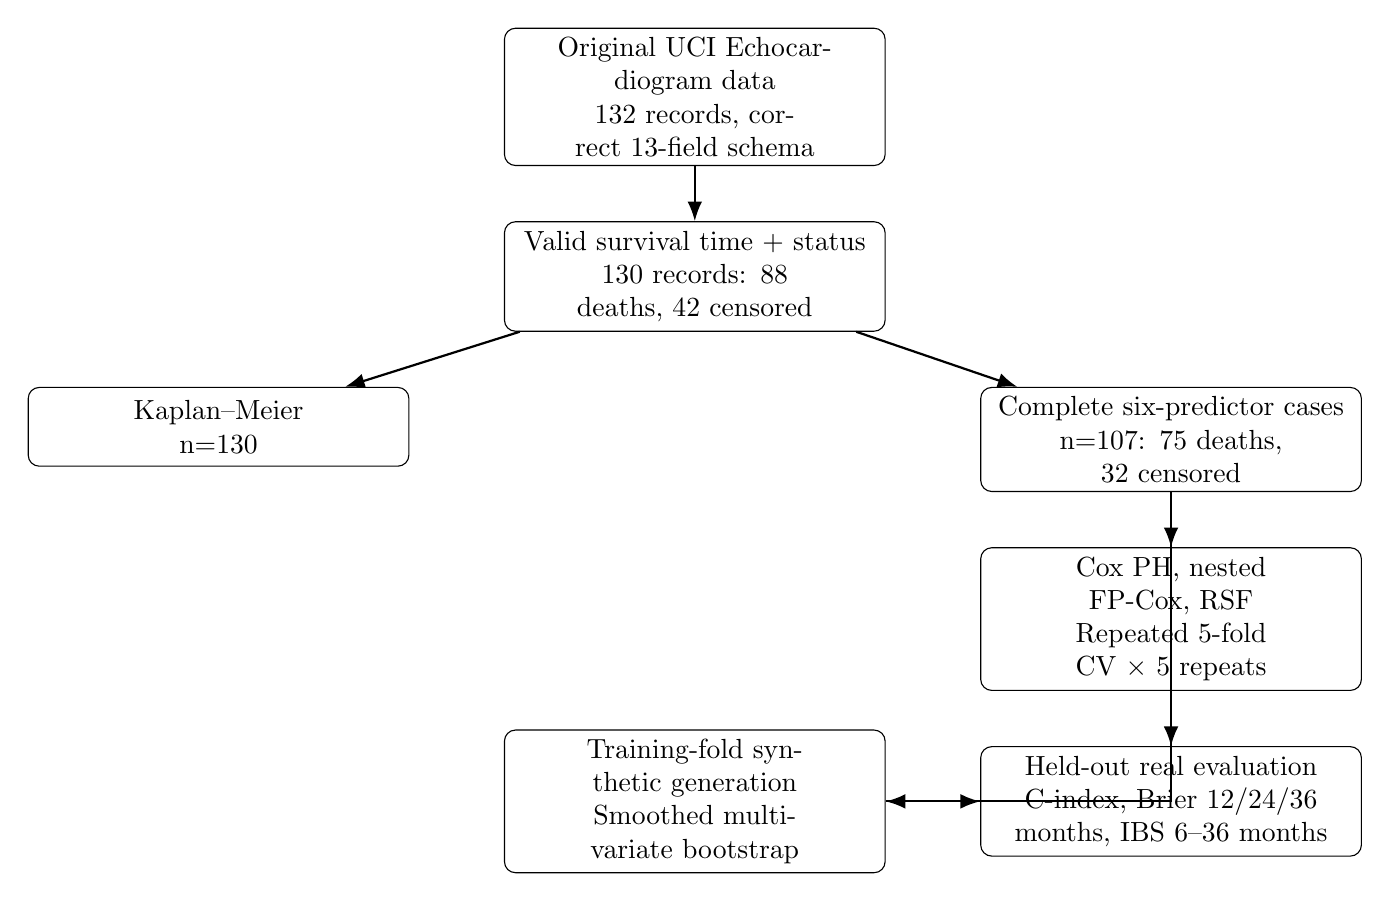
\begin{tikzpicture}[
node distance=7mm and 12mm,
box/.style={rectangle,draw,rounded corners,align=center,text width=4.6cm,minimum height=1.0cm},
arrow/.style={-{Latex[length=2.5mm]},thick}
]
\node[box] (raw) {Original UCI Echocardiogram data\\132 records, correct 13-field schema};
\node[box,below=of raw] (status) {Valid survival time + status\\130 records: 88 deaths, 42 censored};
\node[box,below left=of status] (km) {Kaplan--Meier\\n=130};
\node[box,below right=of status] (cc) {Complete six-predictor cases\\n=107: 75 deaths, 32 censored};
\node[box,below=of cc] (models) {Cox PH, nested FP-Cox, RSF\\Repeated 5-fold CV $\times$ 5 repeats};
\node[box,below=of models] (metrics) {Held-out real evaluation\\C-index, Brier 12/24/36 months, IBS 6--36 months};
\node[box,left=of metrics] (synth) {Training-fold synthetic generation\\Smoothed multivariate bootstrap};
\draw[arrow] (raw) -- (status);
\draw[arrow] (status) -- (km);
\draw[arrow] (status) -- (cc);
\draw[arrow] (cc) -- (models);
\draw[arrow] (models) -- (metrics);
\draw[arrow] (cc) |- (synth);
\draw[arrow] (synth) -- (metrics);
\end{tikzpicture}
\caption{Revised study flow. Synthetic observations were never counted as independent patients and were never used as external validation.}
\label{fig:studyflow}
\end{figure}

\subsection{Kaplan--Meier and Cox proportional hazards analysis}
Kaplan--Meier estimation was applied to the 130 records with valid time/status information \cite{ref29}. A six-variable Cox PH model \cite{ref30} was fitted to the 107 complete cases using Breslow handling of tied event times. Hazard ratios (HRs), 95\% confidence intervals (CIs), and Wald p-values were reported. Proportional-hazards diagnostics were assessed using Schoenfeld-residual time-trend screening for each predictor. Apparent discrimination was summarized by Harrell's C-index. Optimism was additionally assessed by 500 bootstrap resamples; the optimism-corrected C-index equalled the apparent C-index minus mean bootstrap optimism.

\subsection{Fractional-polynomial assessment}
Fractional polynomials were evaluated for age and WMI using the conventional power set $\{-2,-1,-0.5,0,0.5,1,2,3\}$, with power 0 representing the logarithm \cite{ref10,ref36}. FP1 candidates were compared with the all-linear six-variable Cox model using Akaike's Information Criterion (AIC), and FP2 candidates were examined as a sensitivity analysis. To prevent optimistic selection, the predictive FP-Cox analysis re-selected age and WMI powers independently inside every training fold. Linear and selected FP effect curves were generated with other covariates held at their median values.

\subsection{Random Survival Forest and internal validation}
RSF was fitted with \texttt{scikit-survival} \cite{ref38,ref43}. The final confirmation used \texttt{RandomSurvivalForest(n\_estimators=500, min\_samples\_split=10, min\_samples\_leaf=10, max\_features='sqrt')} and fold-specific random seeds. All models were evaluated on the same 25 held-out folds from repeated 5-fold cross-validation (5 repeats; random seed 42). The Cox comparator used \texttt{CoxPHSurvivalAnalysis(alpha=0.0)}. The analysis used full follow-up for the concordance index.

Time-dependent prediction error was evaluated with \texttt{sksurv.metrics.brier\_score} at 12, 24, and 36 months and \texttt{integrated\_brier\_score} over 16 equally spaced points from 6 to 36 months. Inverse probability of censoring weights were estimated from each real training fold. For the 36-month prediction-error calculation, follow-up extending beyond 36 months was administratively censored immediately after the evaluation horizon so that all requested times were strictly inside the observed support required by the software. Lower Brier/IBS values indicate better prediction error, while higher C-index indicates better discrimination.

\subsection{Synthetic-data augmentation experiment}
Synthetic data were retained only as an exploratory methodological component. A smoothed multivariate bootstrap was fitted on the real training fold. Donor rows were sampled with replacement; covariance-aware multivariate Gaussian noise with bandwidth 0.10 was added to survival time, age, fractional shortening, EPSS, LVDD, and WMI, with the covariance matrix regularized toward its diagonal. Generated continuous values were clipped to the observed training-fold ranges and survival time was constrained to remain positive. Event status and pericardial-effusion status were inherited from donor rows. No unobserved clinical variables (for example smoking, cholesterol, diabetes, ejection fraction, or blood pressure) were fabricated for the revised analysis.

Fidelity was assessed on a global 5$\times$ synthetic sample (535 artificial records generated from the 107 real complete cases) using standardized mean differences (SMDs), Kolmogorov--Smirnov (KS) statistics, preservation of binary proportions, Spearman correlation-matrix RMSE, and exact-duplicate checks. Predictive utility was assessed using (i) real-only training, (ii) 5$\times$ synthetic-only training, and (iii) real+1$\times$ synthetic training, with the generator fitted separately within each training fold and all evaluation performed on held-out real observations. Bandwidths 0.05, 0.10, and 0.20 were examined as a sensitivity analysis. Synthetic observations were not interpreted as patients and were not used as external validation \cite{ref40,ref41}.

\subsection{Software, reproducibility, and figure provenance}
The final standard-package confirmation was run with Python 3.11.17, \texttt{scikit-survival} 0.28.0, \texttt{statsmodels} 0.15.0, \texttt{scikit-learn} 1.9.1, \texttt{pandas} 3.0.6, \texttt{NumPy} 2.4.6, and \texttt{SciPy} 1.17.1. The central functions were \texttt{PHReg}, \texttt{CoxPHSurvivalAnalysis}, \texttt{RandomSurvivalForest}, \texttt{concordance\_index\_censored}, \texttt{brier\_score}, and \texttt{integrated\_brier\_score}. Fixed random seeds were used throughout. All quantitative figures in the revised manuscript were generated programmatically from the verified analysis outputs. No generative-AI image system was used to create or alter analysis-derived figures; Figure~\ref{fig:studyflow} is a schematic study-flow diagram.

\section{Results}
\subsection{Analysis population and Kaplan--Meier survival}
Of 132 source records, 130 had valid survival time and vital status. Among these, 88 deaths were observed and 42 records were right-censored. Complete data for the six prespecified model predictors were available for 107 records, including 75 deaths and 32 censored observations.

The corrected Kaplan--Meier curve is shown in Figure~\ref{fig:km}. Estimated survival probabilities were 0.917 at 12 months, 0.701 at 24 months, 0.266 at 36 months, and 0.110 at 48 months. Median observed survival was 29 months. Maximum observed follow-up was 57 months; consequently, the revised manuscript does not report 60-month/5-year survival probabilities.

\begin{figure}[H]
\centering
\includegraphics[width=0.68\linewidth]{figures/kaplan_meier_corrected.png}
\caption{Kaplan--Meier estimate for the 130 records with valid post-MI survival time and event/censoring status.}
\label{fig:km}
\end{figure}

\subsection{Multivariable Cox proportional hazards model}
Table~\ref{tab:cox} presents the corrected six-variable Cox model. None of the predictors reached statistical significance. In particular, the direction of the point estimates should not be interpreted as evidence of protective or harmful effects because the confidence intervals were wide and all p-values exceeded 0.43.

\begin{table}[H]
\centering
\caption{Corrected multivariable Cox proportional hazards model (n=107; 75 deaths).}
\label{tab:cox}
\begin{adjustbox}{max width=\linewidth}
\begin{tabular}{lrrrr}
\toprule
Predictor & HR & 95\% CI lower & 95\% CI upper & p-value \\
\midrule
Age & 0.990 & 0.961 & 1.020 & 0.505 \\
Pericardial effusion & 0.985 & 0.507 & 1.916 & 0.965 \\
Fractional shortening & 0.584 & 0.051 & 6.674 & 0.665 \\
EPSS & 1.021 & 0.970 & 1.075 & 0.431 \\
LVDD & 0.911 & 0.642 & 1.294 & 0.603 \\
Wall-motion index & 0.839 & 0.407 & 1.730 & 0.635 \\
\bottomrule
\end{tabular}
\end{adjustbox}
\end{table}

\begin{figure}[H]
\centering
\includegraphics[width=0.72\linewidth]{figures/cox_forest_corrected.png}
\caption{Hazard ratios and 95\% confidence intervals from the corrected multivariable Cox model. The horizontal axis is logarithmic.}
\label{fig:coxforest}
\end{figure}

The apparent Harrell C-index was 0.532. Across 500 bootstrap resamples, estimated mean optimism was 0.073, yielding an optimism-corrected C-index of 0.459. Schoenfeld-residual screening found no clear evidence of violation of the PH assumption (Table~\ref{tab:ph}). Thus, the principal limitation of the Cox model was weak discrimination rather than a demonstrable PH violation.

\begin{table}[H]
\centering
\caption{Proportional-hazards diagnostic screening.}
\label{tab:ph}
\begin{tabular}{lr}
\toprule
Predictor & Schoenfeld time-trend p-value \\
\midrule
Age & 0.502 \\
Pericardial effusion & 0.963 \\
Fractional shortening & 0.586 \\
EPSS & 0.915 \\
LVDD & 0.930 \\
Wall-motion index & 0.231 \\
\bottomrule
\end{tabular}
\end{table}

\subsection{Fractional-polynomial analysis}
The full-sample all-linear model had AIC 525.149. The best age FP1 form was age$^{-0.5}$ (AIC 525.138), the best WMI FP1 form was WMI$^3$ (AIC 525.046), and the best joint FP1 combination was age$^{-1}$ plus WMI$^3$ (AIC 525.032). The joint improvement relative to the linear model was only 0.117 AIC units. In the joint model, the transformed age and WMI terms were not significant (p=0.487 and p=0.577, respectively). FP2 alternatives had higher AIC and therefore did not improve fit.

\begin{table}[H]
\centering
\caption{Fractional-polynomial model comparison on the complete-case cohort.}
\label{tab:fp}
\begin{tabular}{lrrr}
\toprule
Model & Age power & WMI power & AIC \\
\midrule
Linear age + linear WMI & 1 & 1 & 525.149 \\
Best age FP1 only & -0.5 & 1 & 525.138 \\
Best WMI FP1 only & 1 & 3 & 525.046 \\
Best joint FP1 & -1 & 3 & 525.032 \\
\bottomrule
\end{tabular}
\end{table}

Figures~\ref{fig:agefp} and \ref{fig:wmifp} display the reviewer-requested linear and FP effect curves. The curves are similar across most of the observed predictor range, consistent with the negligible AIC improvement.

\begin{figure}[H]
\centering
\includegraphics[width=0.72\linewidth]{figures/age_linear_vs_fractional_polynomial.png}
\caption{Age effect under the linear Cox specification and the best age FP1 specification. Relative hazards are shown against the median age while other predictors are held at their medians.}
\label{fig:agefp}
\end{figure}

\begin{figure}[H]
\centering
\includegraphics[width=0.72\linewidth]{figures/wmi_linear_vs_fractional_polynomial.png}
\caption{Wall-motion-index effect under the linear Cox specification and the best WMI FP1 specification. Relative hazards are shown against the median WMI while other predictors are held at their medians.}
\label{fig:wmifp}
\end{figure}

Nested selection further showed that the apparent FP forms were unstable: the age/WMI power pair $(-2,3)$ was selected in 7 of 25 folds, $(3,3)$ in 4 folds, and the remaining 14 folds selected 12 other combinations. Therefore, no single nonlinear functional form was reproducible across resamples.

\subsection{Cross-validated model comparison}
Table~\ref{tab:modelcomparison} reports the final standard-package confirmation. All values were obtained on the same 25 held-out real-data folds. Discrimination was weak for all real-data models. RSF produced a mean C-index of 0.446 compared with 0.443 for Cox, while FP-Cox was 0.432. RSF had the lowest IBS (0.167 versus 0.170 for Cox), but the absolute difference was small.

\begin{table}[H]
\centering
\caption{Repeated 5-fold cross-validation (5 repeats) with censoring-aware performance metrics. Mean $\pm$ SD is shown for C-index and IBS; Brier columns are fold means.}
\label{tab:modelcomparison}
\begin{adjustbox}{max width=\linewidth}
\begin{tabular}{lrrrrrr}
\toprule
Training/model & C-index & Brier 12 m & Brier 24 m & Brier 36 m & IBS 6--36 m \\
\midrule
Cox PH, real only & $0.443\pm0.073$ & 0.0815 & 0.2304 & 0.2157 & $0.1698\pm0.0367$ \\
FP-Cox, real only (nested FP) & $0.432\pm0.075$ & 0.0818 & 0.2310 & 0.2181 & $0.1712\pm0.0369$ \\
RSF, real only & $0.446\pm0.080$ & 0.0821 & 0.2278 & 0.2059 & $0.1671\pm0.0349$ \\
Cox PH, synthetic only 5$\times$ & $0.457\pm0.063$ & 0.0816 & 0.2312 & 0.2239 & $0.1718\pm0.0387$ \\
Cox PH, real + 1$\times$ synthetic & $0.457\pm0.079$ & 0.0816 & 0.2327 & 0.2218 & $0.1722\pm0.0385$ \\
\bottomrule
\end{tabular}
\end{adjustbox}
\end{table}

Fold-paired descriptive differences versus real-only Cox were also small (Table~\ref{tab:paired}). We do not attach inferential p-values to these repeated-CV fold differences because folds within repeated cross-validation are not independent observations.

\begin{table}[H]
\centering
\caption{Paired fold-wise differences relative to real-only Cox. Positive $\Delta$C favours the comparator; negative $\Delta$IBS favours the comparator.}
\label{tab:paired}
\begin{adjustbox}{max width=\linewidth}
\begin{tabular}{lrrrr}
\toprule
Comparator & Mean $\Delta$C & Folds with higher C & Mean $\Delta$IBS & Folds with lower IBS \\
\midrule
FP-Cox & -0.0101 & 5/25 & +0.00141 & 4/25 \\
RSF & +0.00338 & 10/25 & -0.00264 & 16/25 \\
Cox + 1$\times$ synthetic & +0.0147 & 14/25 & +0.00243 & 9/25 \\
Synthetic-only 5$\times$ Cox & +0.0145 & 15/25 & +0.00198 & 10/25 \\
\bottomrule
\end{tabular}
\end{adjustbox}
\end{table}

The large gap between apparent and held-out performance observed during the RSF audit indicated overfitting. Cross-validated permutation importance was also unstable: mean C-index changes after permutation ranged from approximately -0.006 for fractional shortening to -0.043 for WMI. Because no feature demonstrated stable positive out-of-sample importance and RSF did not materially outperform Cox, SurvSHAP(t) explanations were not used for clinical inference in the revised manuscript.

\subsection{Synthetic-data fidelity and utility}
The primary fidelity experiment generated 535 artificial records (5$\times$ the 107 complete real records). Table~\ref{tab:synthfidelity} shows close agreement in marginal distributions: the maximum absolute continuous-variable SMD was 0.049 and the largest KS statistic was 0.142. The Spearman correlation-matrix RMSE was 0.035. The real death-event proportion was 0.701 and the synthetic proportion was 0.708. No exact synthetic-to-real duplicate was detected at eight-decimal precision.

\begin{table}[H]
\centering
\caption{Synthetic-data fidelity for the 5$\times$ smoothed multivariate-bootstrap sample.}
\label{tab:synthfidelity}
\begin{adjustbox}{max width=\linewidth}
\begin{tabular}{lrrrr}
\toprule
Variable & Real mean & Synthetic mean & SMD & KS statistic \\
\midrule
Survival & 23.121 & 22.989 & -0.008 & 0.065 \\
Age & 62.594 & 62.989 & 0.045 & 0.097 \\
Fractional shortening & 0.2195 & 0.2189 & -0.005 & 0.052 \\
EPSS & 12.168 & 12.010 & -0.021 & 0.060 \\
LVDD & 4.764 & 4.804 & 0.049 & 0.045 \\
Wall-motion index & 1.359 & 1.353 & -0.014 & 0.142 \\
\bottomrule
\end{tabular}
\end{adjustbox}
\vspace{2mm}
\small Binary proportions: event 0.701 real versus 0.708 synthetic; pericardial effusion 0.187 real versus 0.170 synthetic. Spearman correlation-matrix RMSE=0.035; exact duplicate fraction=0.
\end{table}

Despite satisfactory descriptive fidelity, augmentation did not robustly improve real-patient prediction. Real+1$\times$ synthetic training increased mean C-index from 0.443 to 0.457 but worsened IBS from 0.170 to 0.172; synthetic-only 5$\times$ training showed a similar pattern. Bandwidth sensitivity analysis (0.05, 0.10, 0.20) produced the same qualitative conclusion: the 1$\times$ augmented C-index ranged from 0.455 to 0.457 while IBS remained approximately 0.171, and synthetic-only 5$\times$ C-index ranged from 0.457 to 0.460 with IBS approximately 0.170--0.172. Thus, statistical resemblance did not translate into a consistent predictive advantage.

\section{Discussion}
\subsection{Principal findings}
This revised analysis materially changes the interpretation of the study. First, the UCI Echocardiogram dataset contains 132 original records, not 100,000 patients. The clinically observed outcome is survival after myocardial infarction, not heart failure. Second, after correction of the schema and censoring definition, conventional and flexible survival models showed weak internal discrimination. Third, fractional-polynomial modelling did not provide reproducible evidence of nonlinearity for age or WMI. Fourth, RSF did not materially outperform Cox PH. Finally, synthetic augmentation preserved selected statistical properties but did not provide a robust improvement in held-out real-data performance.

\subsection{Cox modelling and proportional hazards}
No variable in the six-predictor Cox model showed a statistically significant independent association with mortality. This should not be interpreted as evidence that age, ventricular dimensions, contractility measures, or WMI are clinically irrelevant. Rather, the sample is small, confidence intervals are wide, and the number of candidate predictors is substantial relative to the information available. The corrected apparent C-index of 0.532 and optimism-corrected value of 0.459 demonstrate why apparent fit alone is insufficient in this cohort. Repeated cross-validation produced a mean C-index of 0.443, confirming limited generalisability.

The PH diagnostic screening did not identify a clear time-dependent violation among the six prespecified predictors. Consequently, the earlier claim that strongly non-proportional hazards drove the model's behaviour is not supported by the corrected analysis. This illustrates an important methodological point: time-dependent terms should not be introduced by multiplying a predictor by observed survival time, because that directly leaks outcome information into the predictor matrix.

\subsection{Fractional polynomials and nonlinear relationships}
Fractional polynomials are valuable when there is evidence that a continuous covariate's log-hazard relationship departs from linearity \cite{ref10,ref36}. Here, however, the full-sample AIC advantage of the best joint FP1 model over the linear model was only 0.117, and nested resampling selected many different power combinations. The reviewer-requested effect plots similarly show limited separation between linear and FP curves over much of the observed range. These results do not support a stable square-root age effect or a clinically interpretable nonlinear WMI threshold. Reporting this negative result is preferable to selecting one transformation from the full dataset and presenting it as established.

\subsection{RSF, interpretability, and prediction error}
RSF can represent nonlinear interactions without PH assumptions \cite{ref38}, but flexibility can be costly in a cohort of only 107 complete cases. In the common validation framework, RSF's C-index differed from Cox by only +0.003 on average, although its IBS was lower by approximately 0.0026. These differences are too small and inconsistent to justify a claim of clear superiority. Moreover, cross-validated permutation importance was unstable. We therefore do not present SurvSHAP(t), LIME, or SHAP explanations as clinical evidence in the revised manuscript. Explainability methods can clarify how a fitted model behaves, but they cannot rescue a model that has weak or unstable held-out performance.

\subsection{Role of synthetic data}
Synthetic data are not inherently inappropriate in medical research. They can support privacy-preserving development, method testing, or augmentation, particularly where real data are scarce \cite{ref40,ref41}. The methodological issue is whether generated records are clearly distinguished from patients, whether generation preserves clinically relevant joint structure, and whether claimed utility is demonstrated on independent real observations.

The revised smoothed-bootstrap experiment was designed around those principles. The synthetic records showed small SMDs, modest KS statistics, preserved correlation structure, and no exact duplication. Nevertheless, neither synthetic-only nor real+synthetic Cox training improved both discrimination and Brier/IBS performance. Synthetic data therefore remain a secondary methodological experiment rather than an expansion of the clinical cohort. Importantly, they are not external validation and are not used to increase effective sample size for statistical significance.

\subsection{Clinical interpretation and scope}
The correct clinical framing is post-MI survival. The dataset does not contain an observed heart-failure diagnosis, heart-failure subtype, smoking exposure, cholesterol concentration, diabetes status, or blood-pressure measurements as part of the original 13-field UCI schema. Accordingly, the revised manuscript makes no causal or prognostic claims about these unobserved variables. The analysis should be viewed as a methodological reassessment of a small historical echocardiographic dataset rather than a deployable clinical risk model.

The Kaplan--Meier estimates demonstrate substantial mortality over the observed 57-month follow-up, but the multivariable models did not discriminate survivors from non-survivors reliably in held-out data. The results therefore do not support personalised treatment thresholds or clinical deployment. Future work requires a substantially larger contemporary cohort with prospectively defined outcomes, standardized echocardiographic measurements, clinically important covariates, and independent external validation.

\subsection{Strengths and limitations}
A principal strength of the revision is reproducibility: the raw schema, event definition, missing-data handling, cross-validation splits, hyperparameters, package functions, censoring-aware metrics, synthetic-generation procedure, and figure provenance are stated explicitly. All models are compared on identical held-out real folds, and fractional-polynomial selection is nested within training data.

Several limitations remain. The source cohort is small and historical, with missing values in several predictors and only 107 complete cases for multivariable modelling. Complete-case analysis may reduce precision and can introduce bias if missingness is not random. No external clinical cohort was available, so all reported performance is internal validation. Repeated cross-validation reduces dependence on a single split but does not create independent external evidence. The synthetic observations inherit information from the source data and therefore cannot address this limitation. Finally, the weak discrimination and unstable feature importance mean that the models should not be used for clinical decision-making without new external validation.

\section{Conclusion}
After reconstruction of the original UCI Echocardiogram schema and correction of the survival endpoint, the study provides a more cautious assessment of post-MI survival modelling. Among 130 records with valid follow-up, Kaplan--Meier survival declined from 91.7\% at 12 months to 11.0\% at 48 months. In 107 complete cases, no prespecified covariate was independently significant in the multivariable Cox model, and internally validated discrimination was weak. Fractional-polynomial transformations did not materially improve fit or prediction, and RSF provided only a small reduction in integrated Brier score without meaningful improvement in C-index. A carefully controlled synthetic-data experiment preserved selected statistical properties but did not robustly improve held-out real-data performance. These findings support the use of transparent validation and restrained interpretation in small clinical datasets; they do not support treating synthetic records as additional patients, claiming heart-failure prediction, or presenting the current models as externally validated clinical tools.

\section{Declaration}
\subsection*{Author Contributions}
As the first author, Md Abu Sufian led the software development, conceptualisation, design of the methodological framework, data curation, validation, and formal analysis. He contributed to interpreting the results, wrote the original manuscript, reviewed it, and revised it. Wahiba Hamzi was involved in formal analysis, manuscript review, and writing. Mai Ali reviewed and validated the manuscript. Amira Ali provided a critical manuscript review and feedback. Boumediene Hamzi supervised the study, overseeing administrative responsibilities and the investigation, and served as the corresponding author. All authors contributed to the manuscript's development, critical revisions, and final approval.

\subsection*{Funding}
The University Bioscience Lab funded the research.

\subsection*{Data Availability Statement}
The original Echocardiogram data are publicly available from the UCI Machine Learning Repository \cite{ref44} and the public mirror at \url{https://code.datasciencedojo.com/datasciencedojo/datasets/tree/master/Echocardiogram}. The revised primary analyses use the original 132-record dataset; the previously published 100,000-record synthetic extension is not treated as a clinical cohort or as external validation in this revision. Synthetic records used in the augmentation experiment are generated reproducibly from the training data by the supplied code and are not required to reproduce the primary real-data analyses.

\subsection*{Code Availability Statement}
The complete reproducibility workflow includes the corrected UCI parser, Kaplan--Meier analysis, Cox PH model, bootstrap optimism correction, nested fractional-polynomial analysis, RSF analysis, censoring-aware Brier/IBS evaluation, and synthetic-data experiment. Source code is available at \url{https://github.com/datascintist-abusufian/Survival-Analysis}. A frozen revision package containing the scripts and derived outputs is supplied with the revision and will be archived in a DOI-assigning repository (Zenodo) for the final article. No numerical result in this revision depends on undocumented manual calculation.

\subsection*{Figure Provenance}
Figures~\ref{fig:km}, \ref{fig:coxforest}, \ref{fig:agefp}, and \ref{fig:wmifp} were generated programmatically from the verified analysis outputs. Figure~\ref{fig:studyflow} is a schematic diagram of the analysis workflow. No generative image model was used to alter or fabricate data-derived figures.

\subsection*{Acknowledgements}
The authors thank the Research and Technology Department of Imperial College London and Queen Mary University for their indirect support and guidance throughout this study.

\subsection*{Conflicts of Interest}
The authors declare no conflicts of interest related to this study.

\begin{thebibliography}{99}


\bibitem {ref1} Alfadli, K.M. and Almagrabi, A.O., 2023. Feature-limited prediction on the UCI heart disease dataset. Computers, Materials \& Continua, 74(3).
\url{https://doi.org/10.32604/cmc.2023.033603}

\bibitem {ref2} Khan, S.S., Sidney, S., Lloyd-Jones, D.M. and Rana, J.S., 2021. National and global trends of cardiovascular disease mortality, morbidity, and risk. ASPC Manual of Preventive Cardiology, pp.17-33.
\url{https://doi.org/10.1007/978-3-030-56279-3_2}


\bibitem {ref3} Nandal, N., Goel, L. and Tanwar, R., 2022. Machine learning-based heart attack prediction: A symptomatic heart attack prediction method and exploratory analysis. F1000Research, 11, p.1126.
\url{https://f1000research.com/articles/11-1126}


\bibitem {ref4} Giri, B., Agarwal, S.K., Kumari, N., Majumder, R., Gupta, S. and Mitra, A., 2022. Survival prediction of a patient after a heart attack by machine learning. In: 2022 5th International Conference on Contemporary Computing and Informatics (IC3I). IEEE.
\url{https://doi.org/10.1109/IC3I56241.2022.10073329}


\bibitem {ref5} Kaplan, R.M. and Hays, R.D., 2022. Health-related quality of life measurement in public health. Annual Review of Public Health, 43(1), pp.355-73.
\url{https://doi.org/10.1146/annurev-publhealth-052120-012811}

\bibitem {ref6} Tomasoni, D., Adamo, M., Anker, M.S., von Haehling, S., Coats, A.J. and Metra, M., 2020. Heart failure in the last year: progress and perspective. ESC Heart Failure, 7(6), pp.3505-30.
\url{ https://doi.org/10.1002/ehf2.13124}


\bibitem {ref7} Sauerbrei, W., Royston, P. and Look, M., 2007. A new proposal for multivariable modelling of time-varying effects in survival data based on fractional polynomial time-transformation. Biometrical Journal, 49(3), pp.453-73.
\url{ https://doi.org/10.1002/bimj.200610328}

\bibitem {ref8} Berger, U., Gerein, P., Ulm, K. and Schäfer, J., 2000. On the use of fractional polynomials in dynamic Cox models.
\url{https://doi.org/10.5282/ubm/epub.1597}


\bibitem {ref9} Harrell, J., Frank, E. and Harrell, F.E., 2015. Multivariable modelling strategies. Regression Modelling Strategies: With Applications to Linear Models, Logistic and Ordinal Regression, and Survival Analysis, pp.63-102.
\url{https://doi.org/10.1007/978-3-319-19425-7}


\bibitem {ref10} Sauerbrei, W., Perperoglou, A., Schmid, M., Abrahamowicz, M., Becher, H., Binder, H., et al., 2020. State of the art in selecting variables and functional forms in multivariable analysis—outstanding issues. Diagnostic and Prognostic Research, 4, pp.1-18.
\url{https://doi.org/10.1186/s41512-020-00074-3}

\bibitem {ref11}Krzyziński, M., Spytek, M., Baniecki, H. and Biecek, P., 2023. SurvSHAP(t): time-dependent explanations of machine learning survival models. Knowledge-Based Systems, 262, p.110234.
\url{https://doi.org/10.1016/j.knosys.2022.110234}


\bibitem {ref12} Kamran, S., Akhtar, N., Singh, R., Imam, Y., Haroon, K.H., Amir, N., et al., 2021. Association of major adverse cardiovascular events in patients with stroke and cardiac wall motion abnormalities. Journal of the American Heart Association, 10(14), p.e020888.

\url{https://doi.org/10.1161/JAHA.121.020888}


\bibitem {ref13} Rizk, T. and Blankstein, R., 2021. Not all heart attacks are created equal: thinking differently about acute myocardial infarction in the young. Methodist DeBakey Cardiovascular Journal, 17(4), p.60.
\url{https://doi.org/10.14797/mdcvj.345}

\bibitem {ref14} Jiang, N., Wu, Y. \& Li, C. Limitations of using the COX proportional hazards model in cardiovascular research. Cardiovasc Diabetol 23, 219 (2024). \url{https://doi.org/10.1186/s12933-024-02302-2}


\bibitem {ref15} DuBois, Kelly N. Sept. 2019, "DEEP MEDICINE: How Artificial Intelligence Can Make Healthcare Human Again." Perspectives on Science and Christian Faith, vol. 71, no. 3,  pp. 199+. Gale Academic OneFile, \url{link.gale.com/apps/doc/A600162655/AONE?u=anon~dc0be69c&sid=googleScholar&xid=2f3f4f6c}

\bibitem {ref16} Mateusz Krzyziński et al. 2023, SurvSHAP(t): Time-dependent explanations of machine learning survival models, Knowledge-Based Systems, Volume 262, 110234, ISSN 0950-7051, \url{https://doi.org/10.1016/j.knosys.2022.110234}


 \bibitem {ref17}  Krzyziński, M., Spytek, M., Baniecki, H. and Biecek, P., 2023. SurvSHAP(t): Time-dependent explanations of machine learning survival models. \textit{Knowledge-Based Systems}, 262, p.110234. \url{https://doi.org/10.1016/j.knosys.2022.110234}.
    
\bibitem {ref18}  Gao, J., Yousefi, S., Shen, Y., Wang, X., and Liu, H., 2021. DeepSurv: Personalised treatment recommender system using a Cox proportional hazards deep neural network. \textit{BMC Medical Research Methodology}, 21(1), pp.1-15. \url{https://doi.org/10.1186/s12874-021-01234-7}.
    
\bibitem {ref19}  Tang, H., Wang, J., Zhang, Y., and Li, X., 2023. Combining Cox regression and random survival forests for survival analysis. \textit{Journal of Biomedical Informatics}, 135, p.104289. \url{https://doi.org/10.1016/j.jbi.2023.104289}.
    
\bibitem {ref20} Topol, E.J., 2023. High-performance AI models for cardiovascular risk prediction using ensemble learning. \textit{The Lancet Digital Health}, 5(1), pp.1-10. \url{https://doi.org/10.1016/j.ldh.2023.01.003}.
    
\bibitem {ref21}  Li, J., Zhang, T., and Yu, X., 2024. Transformer-based survival analysis for multi-modal medical imaging data. \textit{IEEE Transactions on Medical Imaging}, 43(5), pp.1-12. \url{https://doi.org/10.1109/TMI.2024.3021234}.


\bibitem {ref22} Gelman, A., Carlin, J.B., Stern, H.S., Dunson, D.B., Vehtari, A. and Rubin, D.B., 2013. \textit{Bayesian Data Analysis}. CRC Press.

\bibitem {ref23} Imbens, G.W. and Rubin, D.B., 2015. \textit{Causal Inference in Statistics, Social, and Biomedical Sciences}. Cambridge University Press.


\bibitem {ref24} Sufian, M.A.; Hamzi, W.; Hamzi, B.; Sagar, A.S.M.S.; Rahman, M.; Varadarajan, J.; Hanumanthu, M.; Azad, M.A.K. Innovative Machine Learning Strategies for Early Detection and Prevention of Pregnancy Loss: The Vitamin D Connection and Gestational Health. Diagnostics 2024, 14, 920. \url{https://doi.org/10.3390/diagnostics14090920}

\bibitem {ref25} Sufian, M.A.; Alsadder, L.; Hamzi, W.; Zaman, S.; Sagar, A.S.M.S.; Hamzi, B. Mitigating Algorithmic Bias in AI-Driven Cardiovascular Imaging for Fairer Diagnostics. Diagnostics 2024, 14, 2675. \url{https://doi.org/10.3390/diagnostics14232675}

\bibitem {ref26} Md Abu Sufian, Mingbo Niu, 2025, Hybrid deep learning for computational precision in cardiac MRI segmentation: Integrating Autoencoders, CNNs, and RNNs for enhanced structural analysis,
Computers in Biology and Medicine, Volume 186, 109597, ISSN 0010-4825, 
\url{https://doi.org/10.1016/j.compbiomed.2024.109597}

\bibitem {ref27} Sufian, M.A.; Hamzi, W.; Zaman, S.; Alsadder, L.; Hamzi, B.; Varadarajan, J.; Azad, M.A.K. Enhancing Clinical Validation for Early Cardiovascular Disease Prediction through Simulation, AI, and Web Technology. Diagnostics 2024, 14, 1308. \url{https://doi.org/10.3390/diagnostics14121308}

\bibitem {ref28} Sufian, M.A.; Hamzi, W.; Sharifi, T.; Zaman, S.; Alsadder, L.; Lee, E.; Hakim, A.; Hamzi, B. AI-Driven Thoracic X-ray Diagnostics: Transformative Transfer Learning for Clinical Validation in Pulmonary Radiography. J. Pers. Med. 2024, 14, 856. 
\url{https://doi.org/10.3390/jpm14080856}


\bibitem {ref29} Kaplan-Meier Estimator: Kaplan EL, Meier P. “Nonparametric estimation from incomplete observations.” Journal of the American Statistical Association. 1958;53(282):457–481.
\url{https://doi.org/10.2307/2281868}

\bibitem {ref30} Cox Proportional Hazards Model: Cox DR. “Regression models and life-tables.” Journal of the Royal Statistical Society: Series B (Methodological). 1972;34(2):187–220.
\url{ https://doi.org/10.1111/j.2517-6161.1972.tb00899.x}

\bibitem {ref31} Accelerated Failure Time Models: Klein JP, Moeschberger ML. “Survival Analysis: Techniques for Censored and Truncated Data.” 2nd ed. Springer; 2003.
\url{https://doi.org/10.1007/b97377}


\bibitem {ref32}  Wang Y, Deng Y, Tan Y, Zhou M, Jiang Y, Liu B. A comparison of random survival forest and Cox regression for the prediction of mortality in patients with hemorrhagic stroke. BMC Med Inform Decis Mak. 2023 Oct 13;23(1):215. PMID: 37833724; PMCID: PMC10576378.
\url{https://doi.org/10.1186/s12911-023-02293-2}

\bibitem {ref33}  Mateusz Krzyziński et. al. 2023,  SurvSHAP(t): Time-dependent explanations of machine learning survival models, Knowledge-Based Systems, Volume 262, 2023, 110234, ISSN 0950-7051,
\url{https://doi.org/10.1016/j.knosys.2022.110234}


\bibitem {ref34}  Sauerbrei W, Royston P, Look M. A new proposal for multivariable modelling of time-varying effects in survival data based on fractional polynomial time-transformation. Biom J. 2007 Jun;49(3):453-73. \url{https://doi.org/10.1002/bimj.200610328}


\bibitem{ref35} Cox, D.R. Regression Models and Life-Tables. Journal of the Royal Statistical Society: Series B (Methodological) 1972, 34, 187–220. \url{https://doi.org/10.1111/j.2517-6161.1972.tb00899.x}


\bibitem{ref36} Royston, P.; Altman, D.G. Regression Using Fractional Polynomials of Continuous Covariates: Parsimonious Parametric Modelling. Journal of the Royal Statistical Society: Series C (Applied Statistics) 1994, 43, 429–467. \url{https://doi.org/10.2307/2986270}


\bibitem{ref37} Lundberg, S.M.; Erion, G.G.; Chen, H.; DeGrave, A.; Prutkin, J.M.; Nair, B.; Katz, R.; Himmelfarb, J.; Bansal, N.; Lee, S.I. From Local Explanations to Global Understanding with Explainable AI for Trees. Nature Machine Intelligence 2020, 2, 56–67. \url{https://doi.org/10.1038/s42256-019-0138-9}


\bibitem{ref38} Ishwaran, H.; Kogalur, U.B.; Blackstone, E.H.; Lauer, M.S. Random Survival Forests. The Annals of Applied Statistics 2008, 2, 841–860. \url{https://doi.org/10.1214/08-AOAS169}


\bibitem{ref39} Apley, D.W.; Zhu, J. Visualising the Effects of Predictor Variables in Black Box Supervised Learning Models. Journal of the Royal Statistical Society: Series B (Statistical Methodology) 2020, 82, 1059–1086. \url{https://doi.org/10.1111/rssb.12377}

\bibitem{ref40} Giuffrè M, Shung DL. Harnessing the power of synthetic data in healthcare: innovation, application, and privacy. NPJ Digit Med. 2023 Oct 9;6(1):186. 
\url{https://doi.org/10.1038/s41746-023-00927-3.} 

\bibitem{ref41} Goncalves, A., Ray, P., Soper, B. et al. Generation and evaluation of synthetic patient data. BMC Med Res Methodol 20, 108 (2020). 
\url{https://doi.org/10.1186/s12874-020-00977-1}

\bibitem{ref42}Berger, L., Haberbusch, M., Moscato, F., “Generative adversarial networks in electrocardiogram synthesis: Recent developments and challenges,” Artificial Intelligence in Medicine, vol. 143, p. 102632, Sep. 2023.
\url{https://doi.org/10.1016/j.artmed.2023.102632}



\bibitem{ref43} Pölsterl, S. scikit-survival: A Library for Time-to-Event Analysis Built on Top of scikit-learn. \textit{Journal of Machine Learning Research} 2020, 21, 1--6. \url{https://jmlr.org/papers/v21/20-729.html}

\bibitem{ref44} UCI Machine Learning Repository. Echocardiogram Dataset. University of California, Irvine. \url{https://archive.ics.uci.edu/dataset/38/echocardiogram}

\end{thebibliography}

\end{document}
